\section{Resultados e discussões}
Com base nos testes, valores finais na Tabela~\ref{tabela 2}, foram realizados 65 testes com o intuito de encontrar tendências de ajustes para, assim, encontrar os parâmetros que satisfaçam o que foi pedido. A Tabela~\ref{tabela 2}, nos mostra valores referentes aos resultados finais e que ajustaram. Foram testados números aleatórios tanto para $\rho_0$ (contraste de densidade na superfície), quanto para $\beta$ (fator de contraste de densidade com a profundidade) mantendo apenas a densidade fixa, inalterada. Dessa forma foi possível encontrar os parâmetros com mais eficácia.

    \begin{table}[!h]
    \centering
    \begin{tabular}{|c|c|c|c|}
    \hline
    \multicolumn{1}{|l|}{\textbf{Teste}} & \multicolumn{1}{l|}{\textbf{Contraste $\rho_0$ na superfície}} & \multicolumn{1}{l|}{\textbf{Densidade Fixa}} & \multicolumn{1}{l|}{\textbf{Fator de contraste}} \\ \hline
    \textbf{20}                          & -0.4                                                & -0.4                                         & 80                                               \\ \hline
    \textbf{52}                          & -0.5                                               & -0.4                                         & 10                                               \\ \hline
    \textbf{63}                          & -0.42                                               & -0.4                                         & 60                                               \\ \hline
    \end{tabular}
    \caption{Tabela de valores utilizados nos Testes que ajustaram}
    \label{tabela 2}
    \end{table}


Durante os testes foi reconhecido um padrão entre o aumento do valor $\rho_0$ e o $\beta$. Pode-se aferir que, isso indica: quanto maior o valor de $\rho_0$ (aproximando de 0), maior será o fator de variação do contraste de densidade com a profundidade, necessário para ocorrer um bom ajuste da função hiperbólica.

%%%%%%%%%%%%%%%%%%%%%%%%%%%%%%%%%%%%%%%%%%%%%%%%%%%%%%%%%%%%%%%%%%%%%%%%%%%%%%%%%%%%%%%%%%%%%%%%%%%%%%%%

\subsection{Primeira Questão do Exercício}

Conforme foi apresentado na Tabela~\ref{tabela 2}, os valores encontrados para o ajuste da função hiperbólica com a anomalia gravimétrica constante, serão apresentados com suas respectivas figuras.


\begin{figure}[!h]  
        \centering
        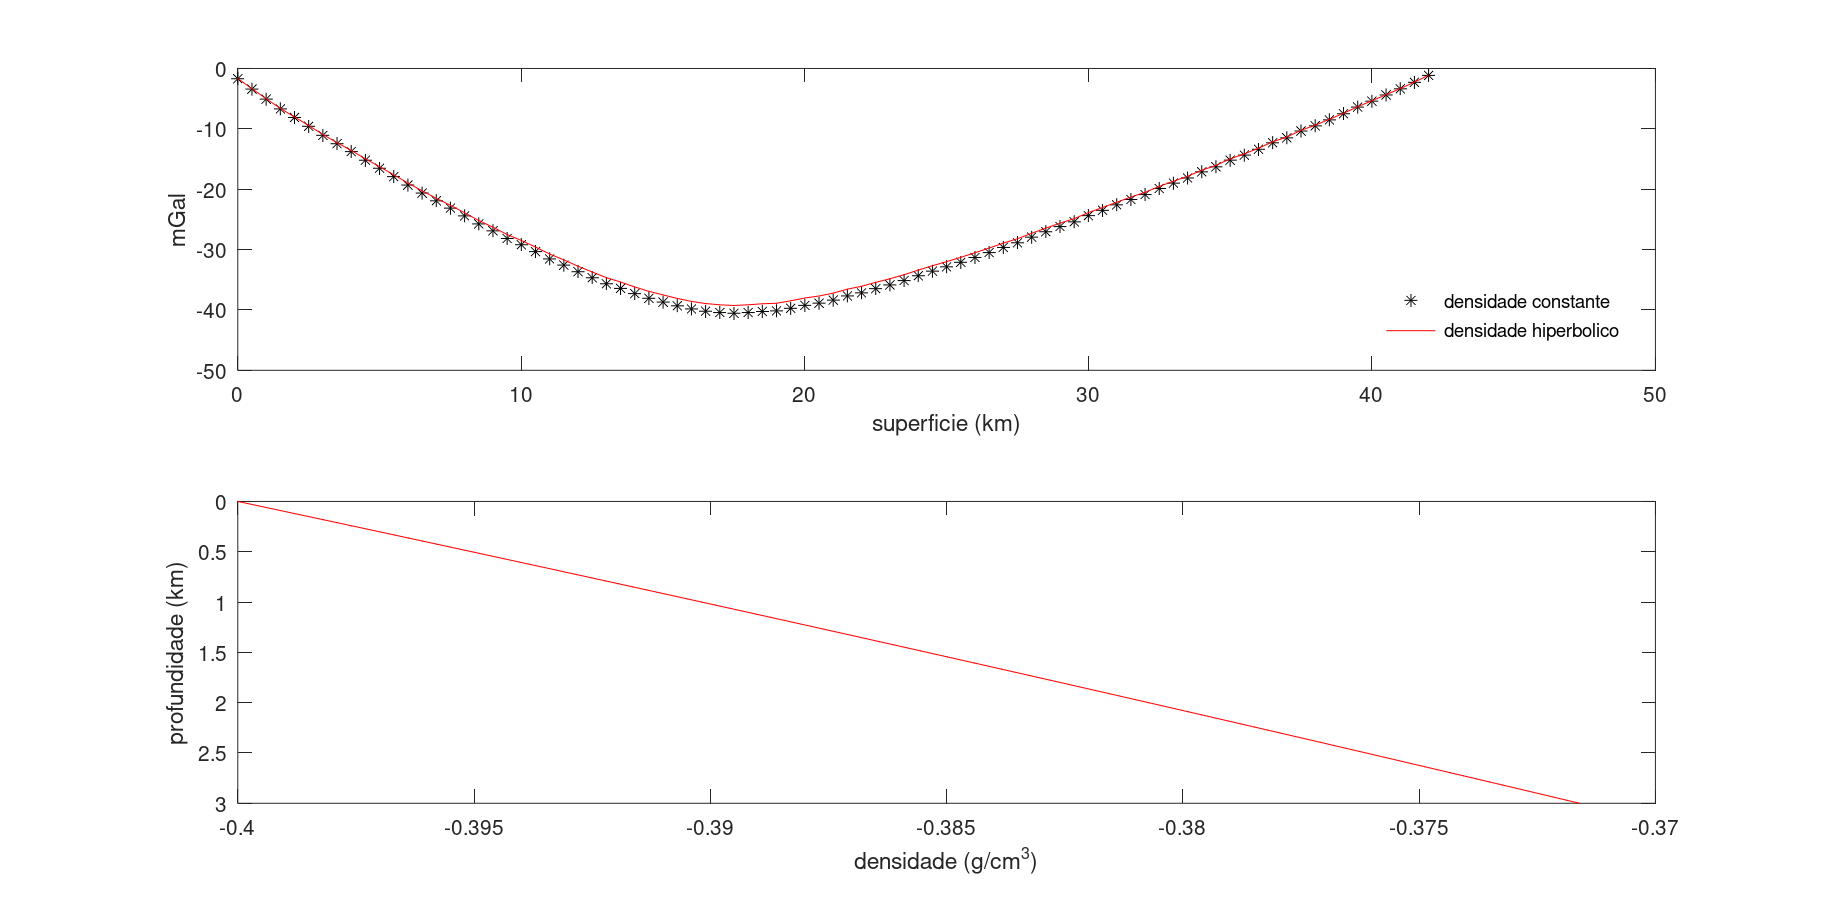
\includegraphics[height=8cm]{figure/Imagens 1a questao/Teste20.png}
        \caption{Ajuste da função hiperbólica com a anomalia gravimétrica, do Teste 20, (Leia-se a 1ª e 2ª imagem como: A e B).}
        \label{Figura 2}
        \end{figure}

A Figura~\ref{Figura 2}, mostra o ajuste da função hiperbólica com a anomalia gravimétrica, resultante do corpo geológico em subsuperfície. A imagem é o resultado do vigésimo teste com os parâmetros: $\rho_0$= -0.4, $\rho$ = -0.4 (Rô aqui representa o contraste de densidade constante) e $\beta$=80. Pode-se notar que a linha em vermelho sobrepõe a linha formada por asterisco, representando um bom ajuste. O fator que informa se os parâmetros utilizados na função, foram bem sucedidos ou não. Além da imagem em si, pode ser também o RMSE. Esse fator nos deu como resultado, do teste 20, o valor de: RMSE=0.728.

%%%%%%%%%%%%%%%%%%%%%%%%%%%%%%%%%%%%%%%%%%%%%%%%%%%%%%%%%%%%%%%%%%%%%%%%%
        \begin{figure}[!h]  
        \centering
        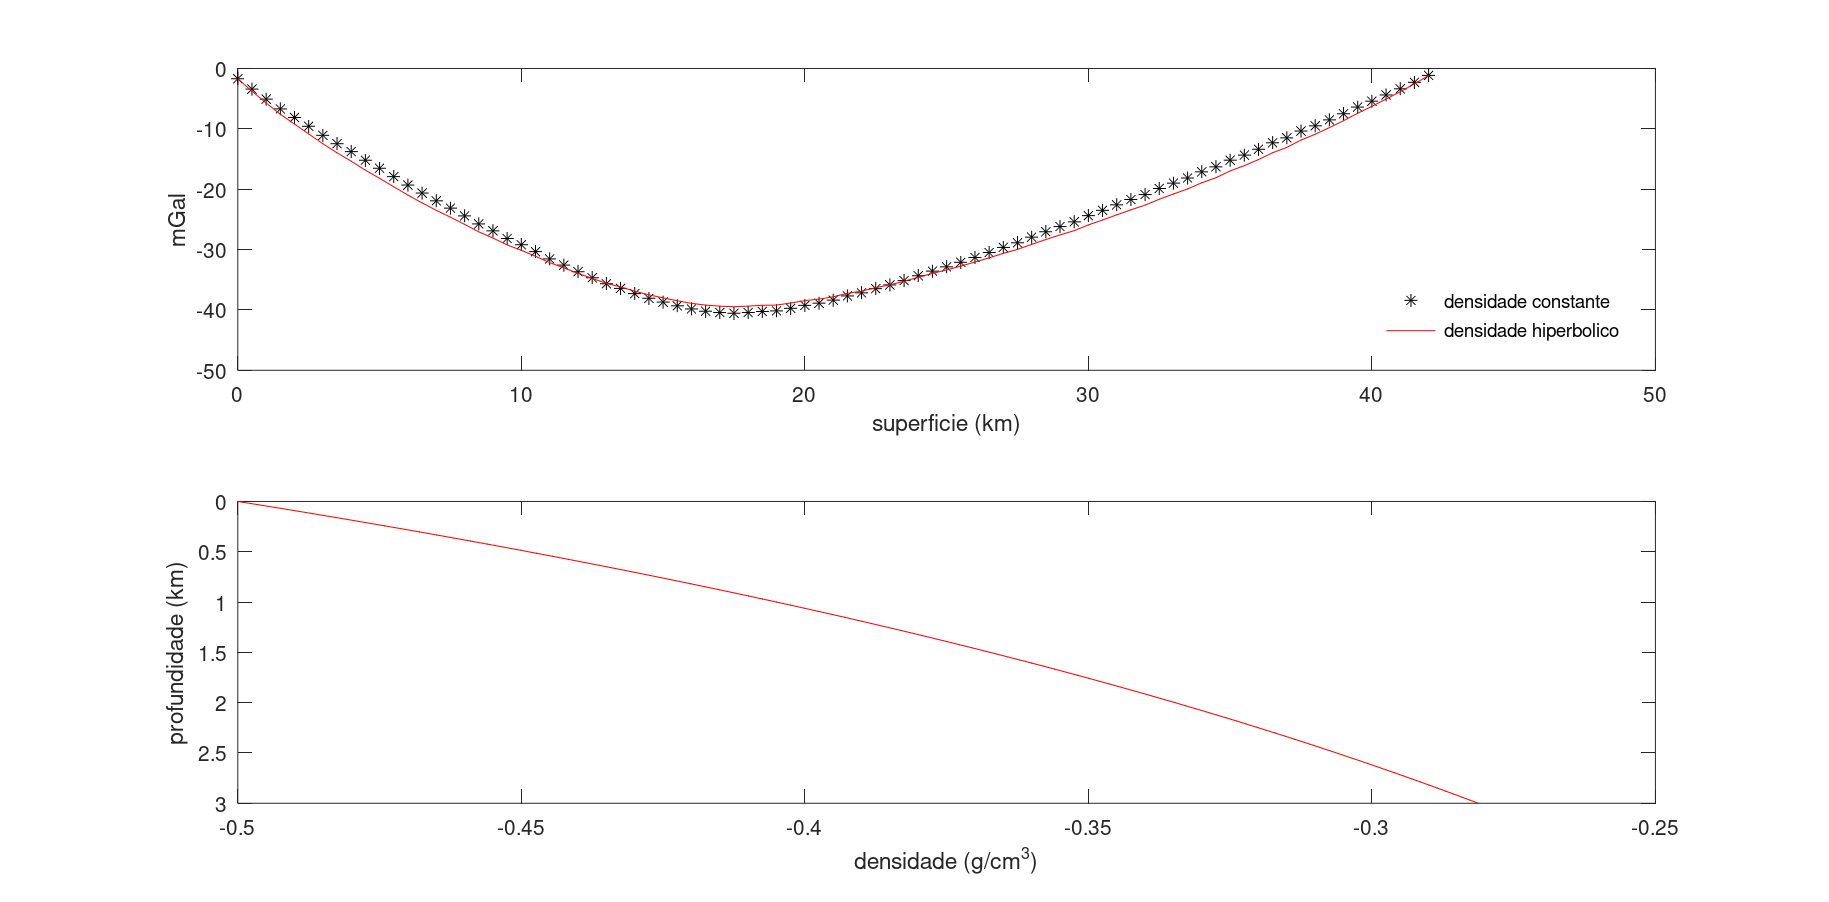
\includegraphics[height=8cm]{figure/Imagens 1a questao/teste52.png}
        \caption{Ajuste da função hiperbólica com a anomalia gravimétrica, do Teste 52 (Leia-se a 1ª e 2ª imagem como: A e B).}
        \label{Figura 3}
        \end{figure}
        
 A Figura~\ref{Figura 3} mostra o ajuste da função hiperbólica com a anomalia gravimétrica resultante do corpo geológico em subsuperfície. A imagem é o resultado do quadragésimo segundo teste com os parâmetros: $\rho_0$= -0.5, $\rho$ = -0.4 (Rô aqui representa o contraste de densidade constante) e $\beta$=10.  Pode-se notar que a linha em vermelho sobrepõe a linha formada por asterisco, representando um bom ajuste. O fator que informa se os parâmetros utilizados na função, foram bem sucedidos ou não, além da imagem em si, pode ser também o RMSE. Esse fator nos deu como resultado o valor de: RMSE=1.350
 
%%%%%%%%%%%%%%%%%%%%%%%%%%%%%%%%%%%%%%%%%%%%%%%%%%%%%%%%%%%%%%%%%%%%%%%%%%
        \begin{figure}[!h]  
        \centering
        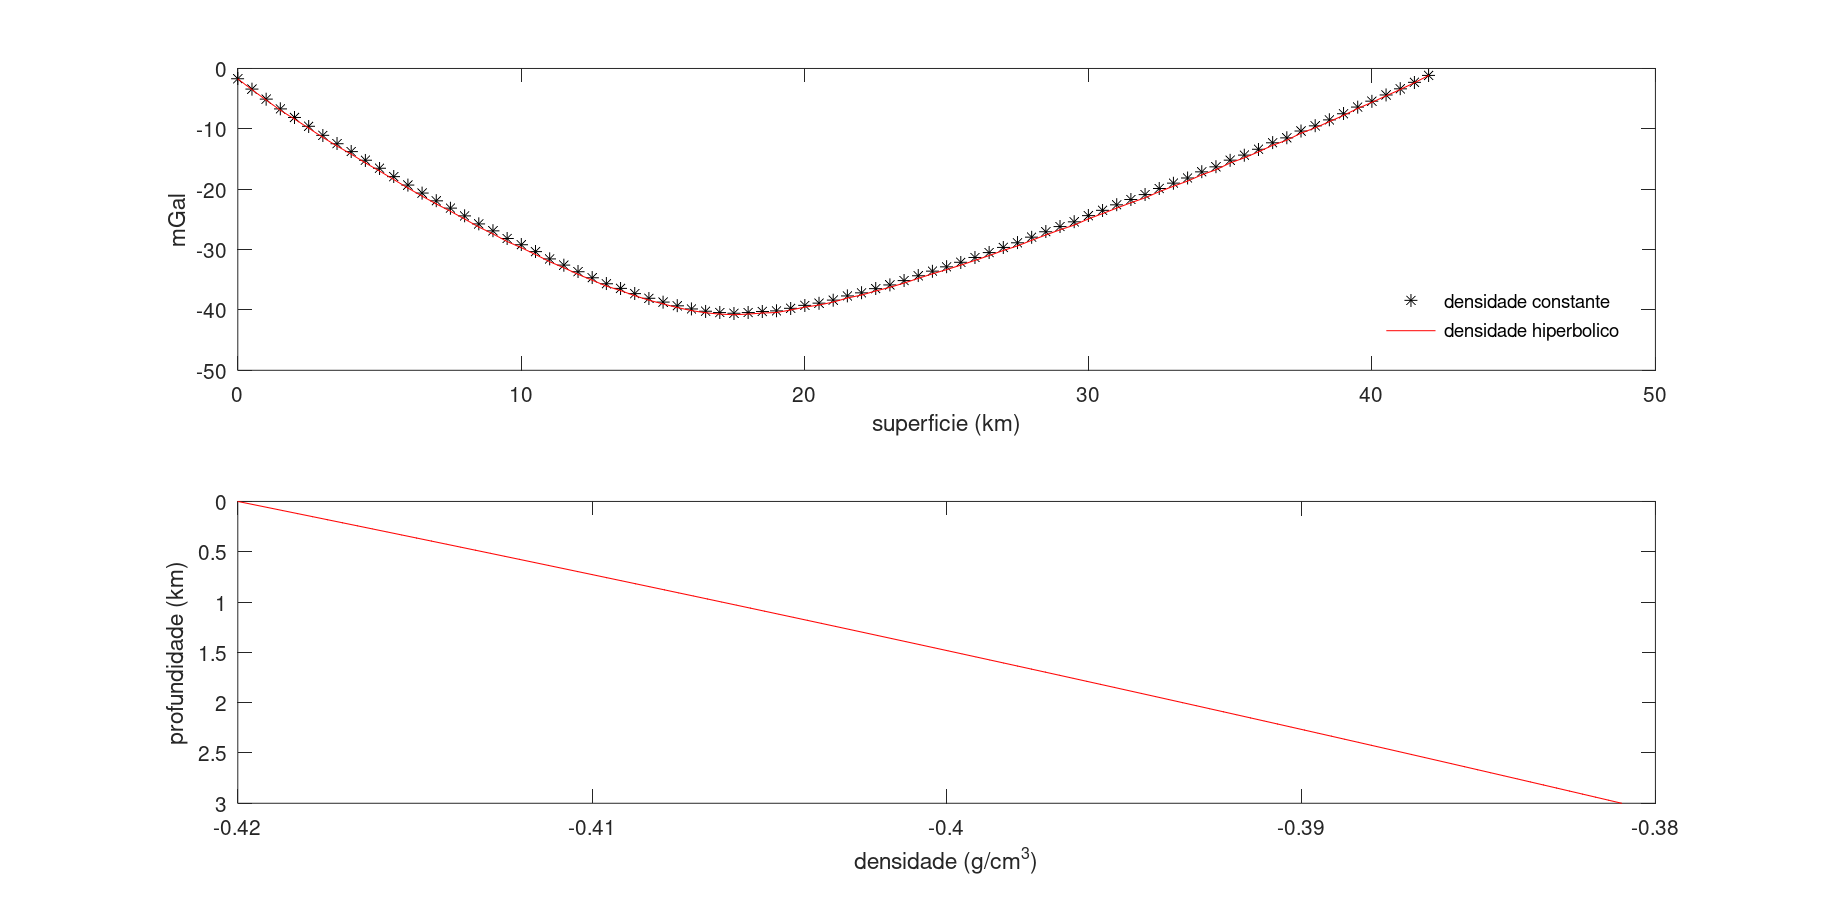
\includegraphics[height=8cm]{figure/Imagens 1a questao/teste63.png}
        \caption{Ajuste da função hiperbólica com a anomalia gravimétrica, do Teste 63 (Leia-se a 1ª e 2ª imagem como: A e B).}
        \label{Figura 4}
        \end{figure}

A Figura~\ref{Figura 4} mostra o ajuste da função hiperbólica com a anomalia gravimétrica resultante do corpo geológico em subsuperfície. A imagem é o resultado do quadragésimo terceiro teste com os parâmetros: $\rho_0$= -0.42, $\rho$ = -0.4 (Rô, aqui representa o contraste de densidade constante) e $\beta$=60. Pode-se notar que a linha em vermelho sobrepõe a linha formada por asterisco, representando um bom ajuste. O fator que informa se os parâmetros utilizados na função, foram bem sucedidos ou não, além da imagem em si, pode ser também o RMSE. Esse fator nos deu como resultado o valor de: RMSE= 0.404, este valor apresentou o melhor ajuste baseado no cálculo do erro.

%%%%%%%%%%%%%%%%%%%%%%%%%%%%%%%%%%%%%%%%%%%%%%%%%%%%%%%%%%%%%%%%%%%%%%%%

\subsection{Segunda Questão do Exercício}

A curva em vermelho na Figura~\ref{Figura 5}b representa a variação do contraste de densidade com a profundidade, gerada pela técnica de densidade hiperbólica. Essa curva indica como o contraste de densidade varia com a profundidade, o que pode ser usado para identificar diferentes camadas geológicas e suas propriedades físicas. Os parâmetros utilizados na Figura~\ref{Figura 5} foram : $\rho_0$ = -0.42, $\rho$ = -0.4 (Rô aqui representa o contraste de densidade constante), $\beta$ = 60 e RMSE = 0.404.

No contexto das anomalias gravimétricas, a curva em vermelho pode ser interpretada como uma representação da distribuição de massa em subsuperfície. Dessa maneira, a função infere que, caso haja uma mudança abrupta na curva, isso pode indicar uma mudança na composição das rochas em subsuperfície. É relevante ressaltar que, tal diferença nos constituintes da rocha, talvez não sejam detectada, através da analise da curva de densidade da função hiperbólica, \cite{silva2006gravity}. Por outro lado, quando a curva apresenta uma variação suave e gradual, isso pode indicar uma camada homogênea de rochas com densidades semelhantes, é o caso de uma bacia sedimentar, como é mostrado na Figura~\ref{Figura 5}b.

De acordo com Silva et al (2006), a lei hiperbólica não pode descrever variações complexas de densidade, como as encontradas na Bacia do Recôncavo. Isso sugere que a variação da densidade com a profundidade pode ser mais complexa do que uma simples função hiperbólica e pode estar relacionada a outras características geológicas da bacia sedimentar. Portanto, o autor destaca a importância de considerar informações adicionais sobre o ambiente geológico da bacia sedimentar para obter estimativas mais precisas da variação da densidade com a profundidade. O documento também apresenta um método para incorporar informações prévias sobre suavidade e profundidade do embasamento para melhorar a estabilidade das soluções.
         \begin{figure}[!h]  
                \centering
                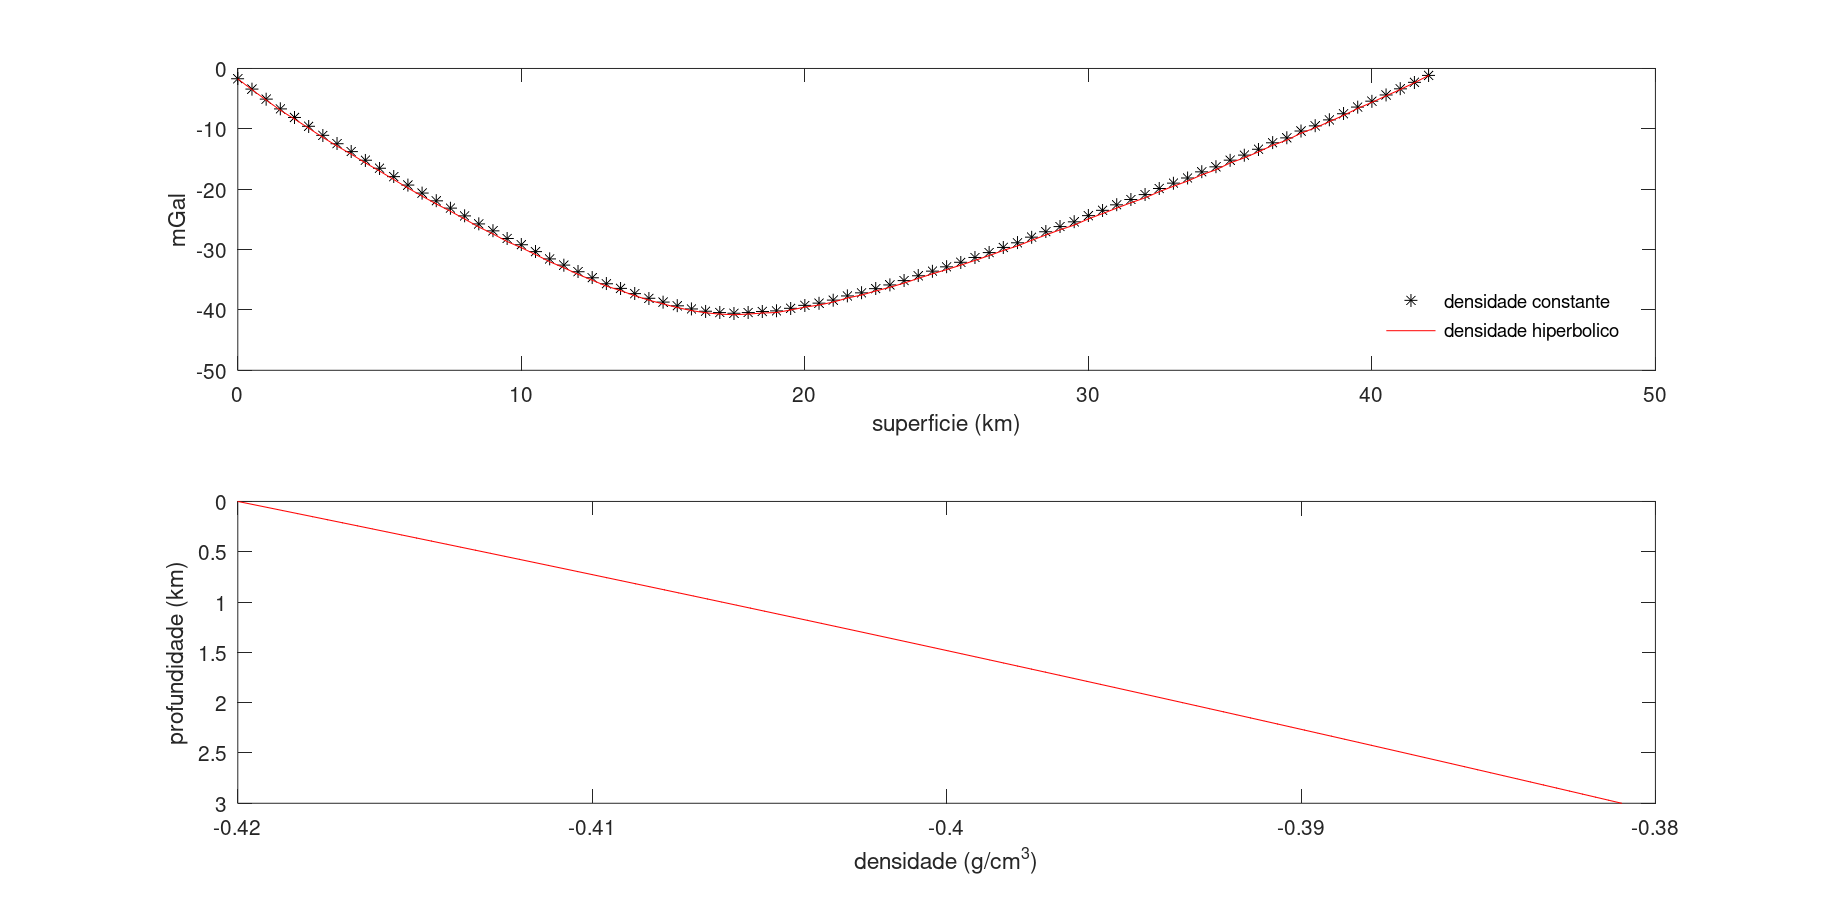
\includegraphics[height=8cm]{figure/Imagens 1a questao/teste63.png}
                \caption{Representação do ajuste e a variação da densidade com a profundidade, referente ao Teste 63 (Leia-se a 1ª e 2ª imagem como: A e B).}
                \label{Figura 5}
            \end{figure}

%\vspace{2.cm}
%%%%%%%%%%%%%%%%%%%%%%%%%%%%%%%%%%%%%%%%%%%%%%%%%%%%%%%%%%%%%%%%%%%%%%%%

\subsection{Terceira Questão do Exercício}

Os principais fatores que podem contribuir para um não ajuste entre as curvas, em questão, são: a presença de heterogeneidades na subsuperfície e a variação da densidade das rochas com a profundidade. Esses fatores podem afetar as anomalias gravimétricas e causar curvas que não se ajustam perfeitamente aos dados observados. No ponto de vista, observado pelo autor deste relatório, notou-se que quanto maior for a distância dos valores entre o fator de contraste de densidade com a profundidade e o contraste de densidade hiperbólico, maior será a dificuldade, das curvas, ajustarem-se. A Figura~\ref{Figura 6}a exemplifica bem, oque foi dito. Os parâmetros utilizados foram : $\rho_0$ = -0.42, $\rho$ = -0.4 (Rô aqui representa o contraste de densidade constante), $\beta$ = 5 e RMSE = 7.047.

 \begin{figure}[!h]  
        \centering
        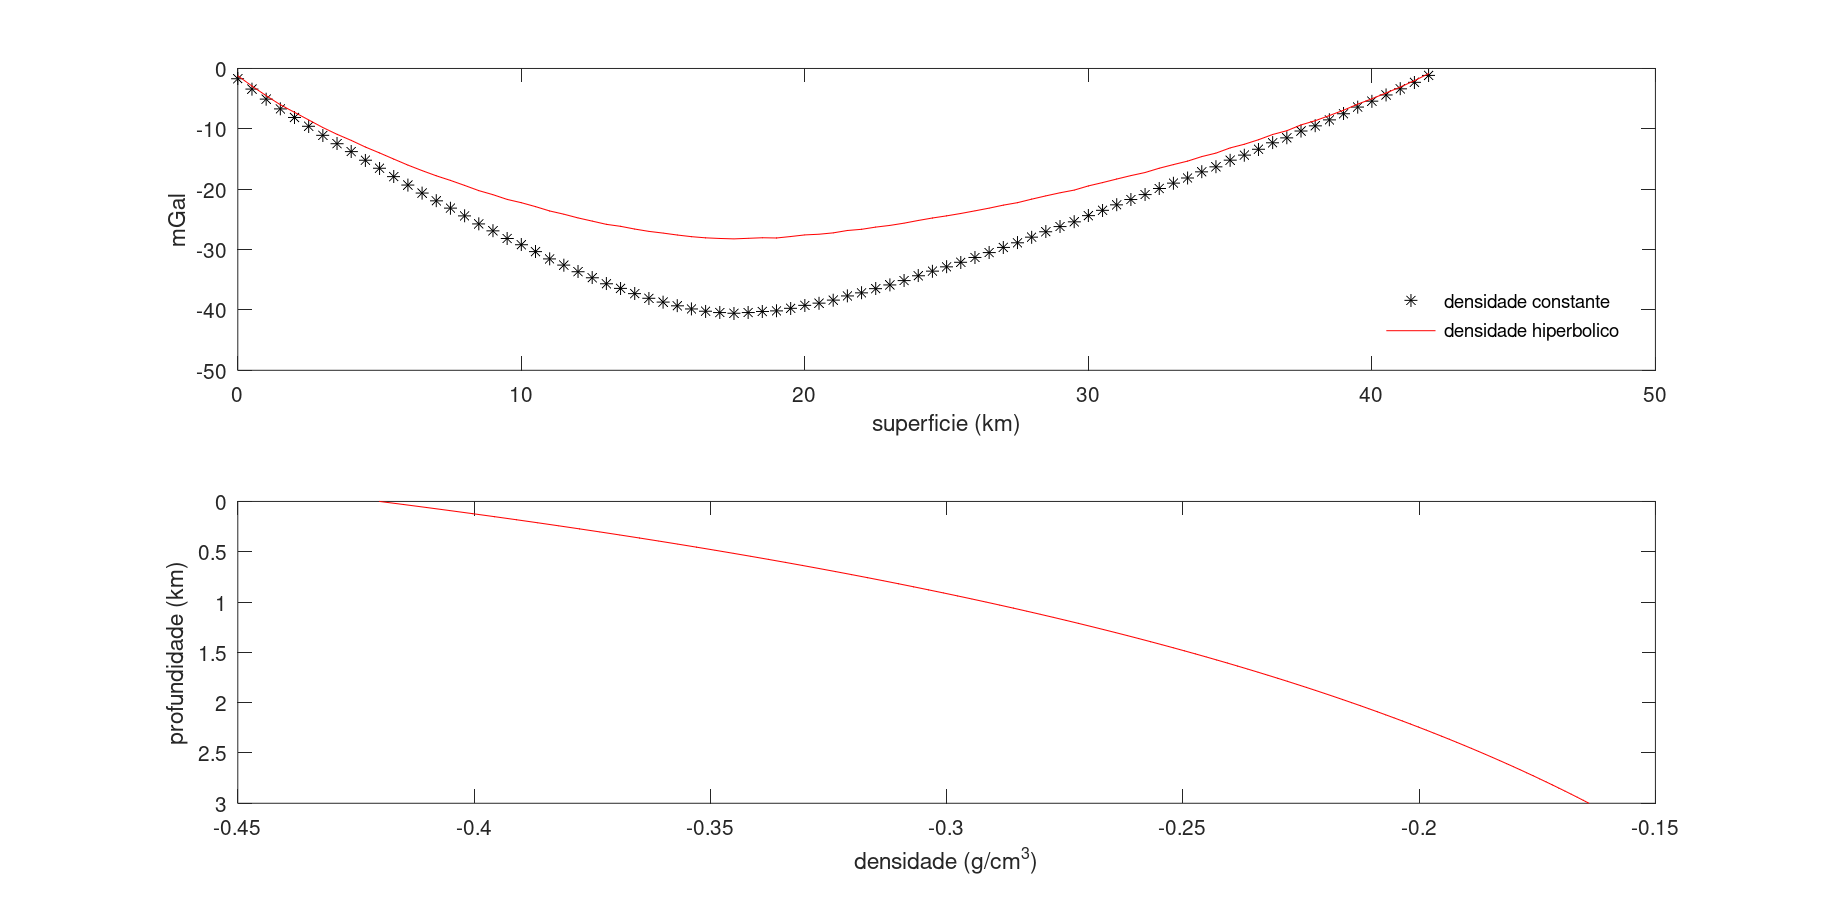
\includegraphics[height=8cm]{figure/Imagens 1a questao/Teste 64.png}
        \caption{Representação do ajuste e a variação da densidade com a profundidade, referente ao Teste 64 (Leia-se a 1ª e 2ª imagem como: A e B).}
        \label{Figura 6}
    \end{figure}

%%%%%%%%%%%%%%%%%%%%%%%%%%%%%%%%%%%%%%%%%%%%%%%%%%%%%%%%%%%%%%%%%%%%%%%
\vspace{6.cm}
\subsection{Quarta Questão do Exercício}

Como já foi a bordado nas questões anteriores, as condições dos ambientes geológicos podem apresentar diferentes propriedades físicas das rochas que influenciam o comportamento das curvas de anomalias gravimétricas. Por exemplo, em ambientes com rochas homogêneas e densidade constante, é mais provável que as curvas se ajustem aos dados observados, como é ilustrado pela Figura~\ref{Figura 7}. Os parâmetros utilizados foram : $\rho_0$ = -0.43, $\rho$ = -0.4 (Rô aqui representa o contraste de densidade constante), $\beta$ = 40 e RMSE = 0.608.


        \begin{figure}[!h]  
                \centering
                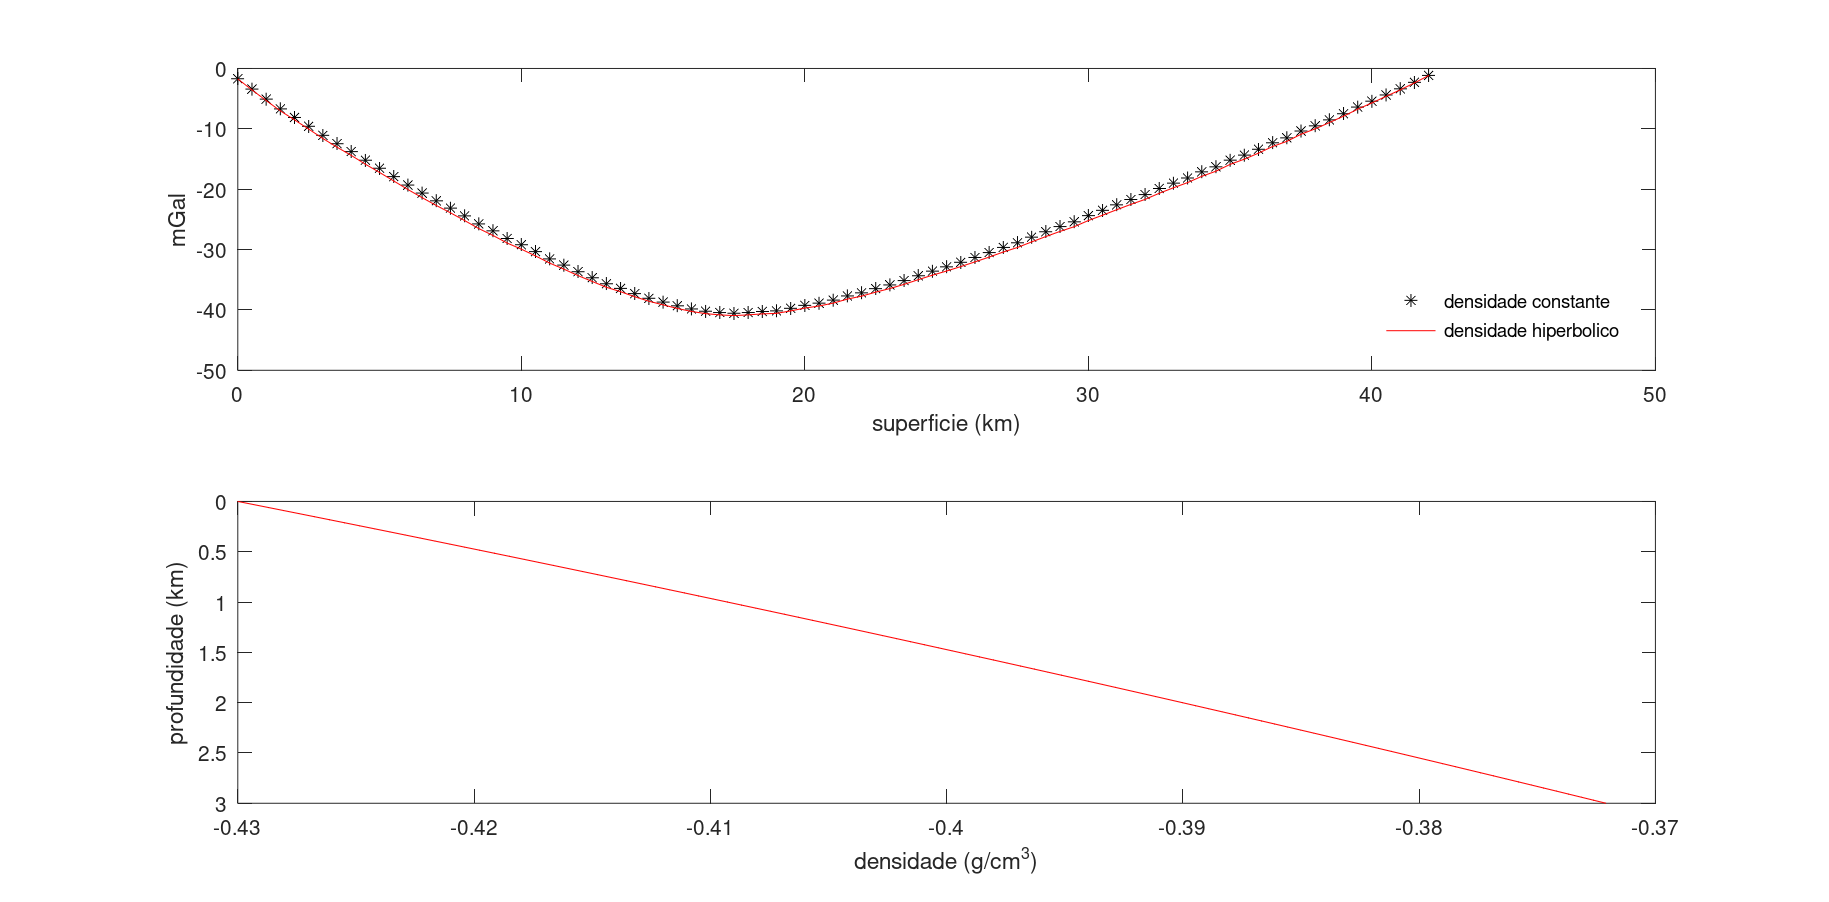
\includegraphics[height=8cm]{figure/Imagens 1a questao/teste62.png}
                \caption{Representação do ajuste e a variação da densidade com a profundidade, referente ao Teste 62 (Leia-se a 1ª e 2ª imagem como: A e B).}
                \label{Figura 7}
            \end{figure}


\vspace{0.65cm}

Já em ambientes com rochas heterogêneas e densidade variável, é mais provável que as curvas não se ajustem perfeitamente aos dados observados, como é mostrado na Figura~\ref{Figura 8}. Os parâmetros utilizados foram : $\rho_0$ = -0.42, $\rho$ = -0.4 (Rô aqui representa o contraste de densidade constante), $\beta$ = 1 e RMSE = 17.453

        \begin{figure}[!h]  
                \centering
                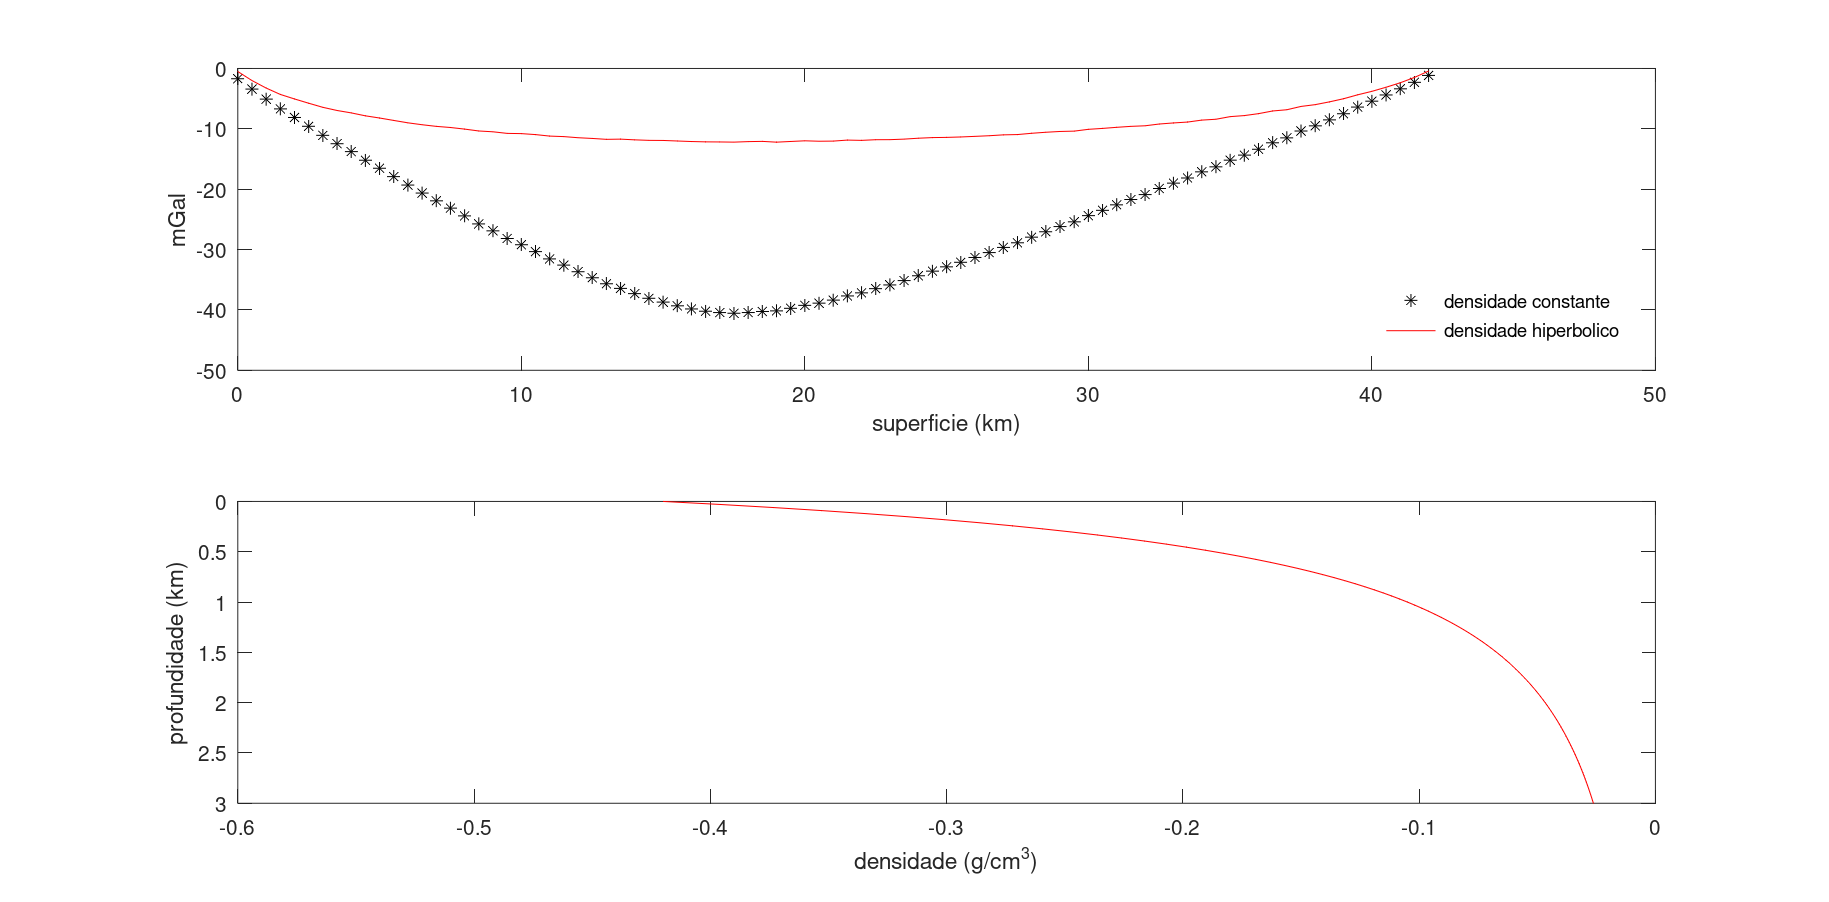
\includegraphics[height=8cm]{figure/Imagens 1a questao/Teste 65.png}
                \caption{Representação do ajuste e a variação da densidade com a profundidade, referente ao Teste 65 (Leia-se a 1ª e 2ª imagem como: A e B).}
                \label{Figura 8}
        \end{figure}
        
 Com esses exemplos em imagens pode-se concluir que, é importante levar em consideração as condições dos ambientes geológicos ao interpretar as curvas de anomalias gravimétricas e realizar testes para avaliar a precisão dos modelos utilizados.

